\documentclass[thesis=bachelor,faculty=cb]{hsmw-thesis}
\usepackage{listings}
\usepackage{xcolor}
\usepackage{float}
\usepackage{amsfonts}
\usepackage{hyperref}
\title[Research on the certificate-based updating of embedded control systems]{Untersuchungen zur zertifikatsbasierten Aktualisierung von verteilten Steuerungssystemen}
\author{Marc}{Ulbricht} 
%<signatur-schildbach.pdf>
\submissiondate{2022}[8][4]
\faculty{Angewandte Computer- und Biowissenschaften}
\courseofstudy[Applied Computer Science]{Angewandte Informatik}
\seminargroup{IF17wI-B}
\examiner[Prof. Dr.-Ing.]{Thomas Beierlein}
\addexaminer{Andreas Weger}[M.Sc.]
\abstract{In dieser Bachelorarbeit soll ein System, welches die Authentizität und Unversehrtheit einer Firmwareaktualisierung vor Installation auf dem Zielgerät sicherstellt, theorisiert und umgesetzt werden.
	Hierfür werden Verfahren herangezogen, welche auf möglichst lange Sicht sicher bleiben, aber gleichzeitig immer größer werdende Firmwarepakete trotzdem effizient verarbeiten sollen.
	Dabei ist zu priorisieren, dass möglichst wenig Änderungen am Zielgerät vorgenommen werden, da sich diese im bereits ausgelieferten Zustand befinden.
	Des Weiteren soll sich der bisherige Ablauf einer Aktualisierung nicht merkbar verändern.}
\lstset{basicstyle=\ttfamily,
	keywordstyle=\color{blue}\ttfamily,
	showstringspaces=false,
	stringstyle=\color{orange}\ttfamily,
	commentstyle=\color{red}\ttfamily,
	morecomment=[l][\color{magenta}]{\#},
	breaklines=true,
	frame=single
}
\hypersetup{hidelinks}
\begin{document}
\lstlistoflistings
\chapter{Einleitung}
Sicherheit und vor allem Sicherheit im Internet ist eines der großen Themen dieser Zeit, gerade jetzt, da immer mehr Geräte und nicht nur der Heimcomputer mit dem Internet verbunden sind. Bei einer Firma wie Iseg, welche Hochspannungsversorgungen für Wissenschaft und Industrie herstellt ist Sicherheit umso wichtiger. Erst vor kurzem wurde eine Sicherheitslücke \cite{0Day} im Diagnose-Tool von Microsoft Office \enquote{Microsoft Support Diagnostic Tool (MSDT)} entdeckt.
Das Öffnen eines Word-Dokumentes und das leichtfertige Deaktivieren der \enquote{geschützten Ansicht} reicht dem Angreifer bereits aus, um Code nachzuladen und PowerShell-Code auszuführen.
Der Angreifer kann sich so möglicherweise Rechte verschaffen und das ganze System übernehmen. Ähnliches könnte auch passieren, wenn eine Firmwareaktualisierung auf dem Weg zum Kunden abgefangen wird. Sie könnte so verändert werden, dass einem Angreifer nach der Installation voller Zugriff auf das Gerät möglich ist. Durch solch eine Veruntreuung eines Hochspannungsgerätes ließe sich enormer Schaden anrichten. Deshalb sollten externe Dateien wie zum Beispiel Firmwareaktualisierungen verifiziert werden, bevor sie am Gerät Verwendung finden können.
\newpage
\section{Aufgabenstellung}
Ziel dieser Bachelorarbeit ist die Planung und Entwicklung einer Softwarelösung, welche die von der Firma Iseg bereitgestellten Firmwareaktualisierungen signiert und verifiziert. Die Updates sollen vor dem Verteilen signiert werden und vor der Installation automatisch auf Echtheit und Unversehrtheit geprüft werden. Dabei soll es trotzdem möglich bleiben ein Update auch ohne gültige Verifikation durchzuführen, sollte ein Fehler beim Verifizieren auftreten, oder sich die Softwarelösung auf dem Gerät durch z.B. Alter des Gerätes nicht umsetzen lassen und keine Möglichkeit zum Verifizieren bestehen.
\noindent
Hier könnte dem Endkunden durch entsprechendes visuelles Feedback die Möglichkeit gegeben werden, zu entscheiden, ob und wie mit dem Update weiter verfahren werden soll. Dies dürfte allerdings die einzig mögliche merkbare Abweichung vom derzeitigen Aktualisierungsprozess sein.
Des Weiteren sind die Zielgeräte bereits ausgeliefert, daher ist ein Weg zu finden, die Softwarelösung möglichst einfach zu verteilen. 
Zu Beginn soll aber zunächst ein geeignetes Signaturverfahren erörtert werden, welches möglichst große Sicherheit bietet, ohne merklich die Geschwindigkeit eines Updates zu mindern.
\chapter{Grundlagen}
Dieses Kapitel gibt einen Einblick in die theoretischen Grundlagen von Signaturverfahren. Außerdem sollen das Iseg Updateverfahren sowie die beim Testen der Signaturverfahren verwendete Hardware vorgestellt werden.
\section{Digitale Signaturen}
Digitale Signaturverfahren sind sogenannte Asymmetrische Kryptosysteme, auch \enquote{Public-Key-Verfahren} genannt. So erstellt ein Benutzer mithilfe eines mathematischen Verfahrens, worin sich die einzelnen Signaturverfahren unterscheiden, ein Schlüsselpaar aus einem geheimen und einem öffentlichen Schlüssel. Diese sollen in dieser Arbeit fortan \enquote{private-key} und \enquote{public-key} heißen. Mithilfe des private-key kann der Benutzer seine Daten eindeutig signieren. Der public-key dient dazu diese Signatur zu prüfen und kann den Benutzer somit als ursprünglichen Besitzer der Daten authentifizieren. 
\begin{figure}[H]
	\centering
	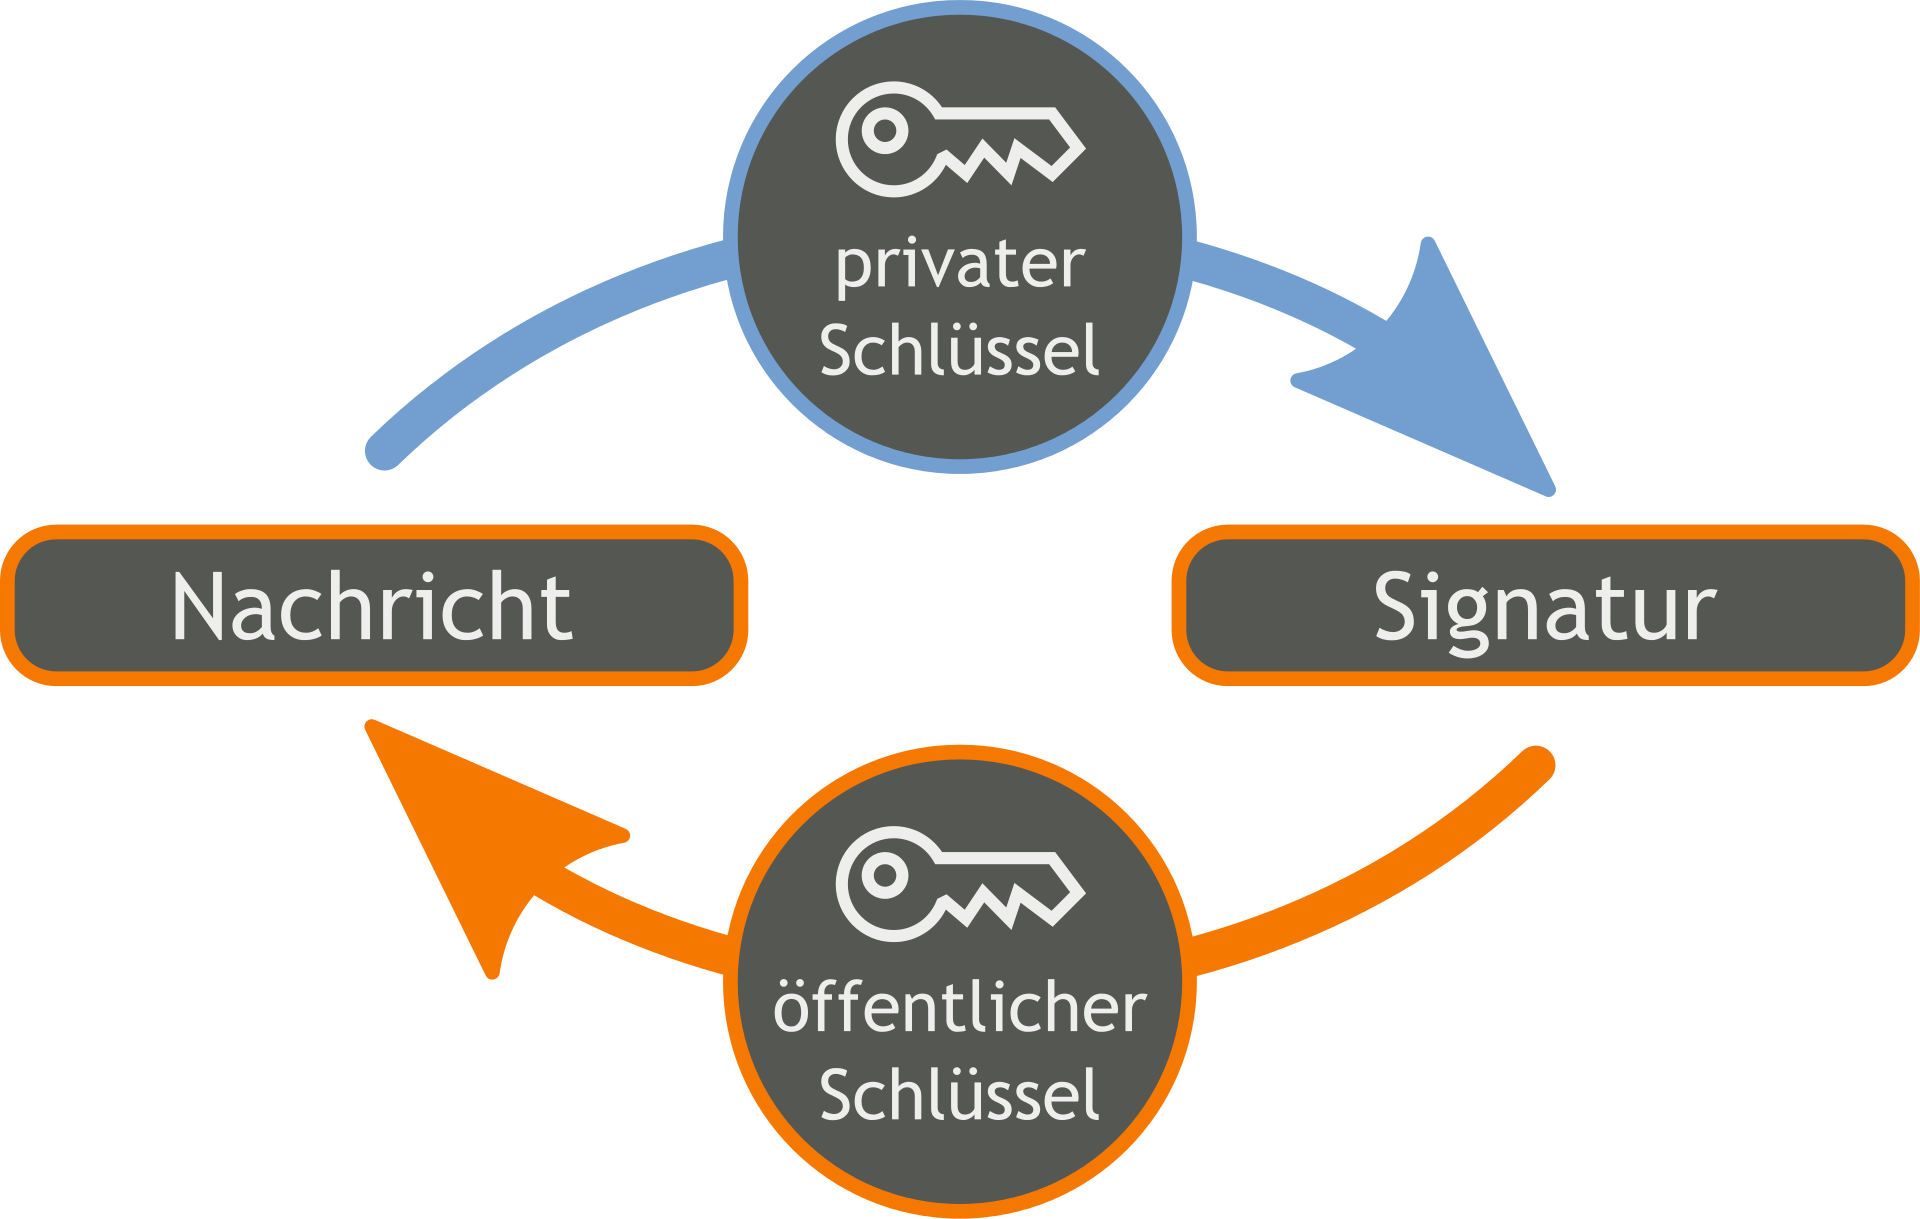
\includegraphics[scale=0.09]{images/Orange_blue_digital_signature_de.svg.png}
	\caption{Simplifizierte Veranschaulichung zu Signaturverfahren}{Quelle: \url{ https://upload.wikimedia.org/wikipedia/commons/2/29/Orange_blue_digital_signature_de.svg}}
\end{figure}
Darin liegt auch der Vorteil eines Asymmetrischen Kryptosystems. Sender und Empfänger müssen vorher kein gemeinsames Geheimnis ausmachen, da nur eine Partei den Ursprung und die Echtheit ihrer Daten darlegen will. Somit lassen sich zwar keine sensiblen Daten sicher verschlüsseln, aber dies wäre auch nicht zielführend für diese Arbeit, da die Firmwareaktualisierungen der Firma Iseg auch öffentlich zugänglich sind und nur ihre Authentizität und Unversehrtheit vor der Installation nachgewiesen werden muss. \\
\\[1cm]
In folgenden Teilkapiteln sollen nun die mathematischen Grundlagen der Schlüsselerzeugung ausgewählter Verfahren aufgezeigt werden.
\\[1cm]´
\section{RSA}
RSA ist ein asymmetrisches Kryptographieverfahren, welches 1978 von Ronald Rivest, Adi Shamir und Leonard Adleman veröffentlicht wurde. Aus ihren Nachnamen erschließt sich hierbei auch der Name des Verfahrens "RSA". 

Die Vorstellung von RSA findet auf Grundlage der Vorlesungsunterlagen \cite{RSA} zu Prof. K. Dohmens Kurs \enquote{Grundlagen der Kryptologie} statt.  
\\[1cm]
Bei diesem Verfahren werden ein public-key und ein private-key generiert. Der public-key besteht dabei aus dem RSA-Modul $n$ sowie dem Verschlüsselungsexponenten $e$. Der private-key enthält ebenfalls $n$ und den Entschlüsselungsexponenten $d$.
Die Namen der Exponenten scheinen möglicherweise unsinnig, da beim Signieren der private-key verwendet wird. Dies hat jedoch den Grund, dass das Signieren die Operationen des Verschlüsselns einer Nachricht in umgekehrter Reihenfolge durchführt. So würde beim Verschlüsseln mit dem public-key agiert werden und der Name Verschlüsselungsexponent wäre sinnvoll.
\\[1cm]
Zum Erstellen der Schlüssel werden zunächst zwei große zufällige Primzahlen $p$ und $q$ generiert, für welche $p \neq q$ gilt. Der RSA-Modul $n$ lässt sich nun als $n = p \times q$ berechnen. Außerdem wird \begin{math}\phi(n) = (p-1)\times(q-1) \end{math} berechnet.
$\phi()$ meint die Eulersche $\phi$-Funktion, welche einer natürlichen Zahl $n$ die Anzahl aller natürlicher Zahlen von $1$ bis $n$, welche zu $n$ teilerfremd sind, zuordnet. Hierbei handelt es sich um einen Spezialfall, da $p$ und $q$ Primzahlen sind. Somit wäre $q$ zu den Zahlen von $1$ bis $q-1$ teilerfremd und $\phi(q)$
lässt sich als $q-1$ darstellen. Wird dies auch bei $p$ angewandt ergibt sich für $\phi(n)$ die oben genannte Definition $\phi(n) = (p-1) \times (q-1)$. Danach wird der Verschlüsselungsexponent $e$ so gewählt, dass $e \in \mathbb{N}$, $1 < e < \phi(n)$ gilt und dass $e$ und $\phi(n)$ teilerfremd
sind. Der public-key ist somit berechnet und lässt sich als folgendes Tupel $(n, e)$ darstellen. 
\\[1cm]
Für den private-key fehlt nun noch der Entschlüsselungsexponent $d$, welcher sich aus $e \times d = 1 ( \mod \phi(n))$ berechnen lässt, vorausgesetzt $d \in \mathbb{N}$ und $d$ erfüllt die Vorgabe $1 < d < \phi(n)$.
Der private-key $(n, d)$ ist einsatzbereit, nun sollten sicherheitshalber $p$, $q$ und $\phi(n)$ gelöscht werden um mögliche Spuren von public und private-key zu verwischen. Eine Nachricht $m$ soll nun signiert werden. Zunächst wird ein Hash der Nachricht ($Hash(m)$) erstellt, da so die Größe der Nachricht keinen
Einfluss auf die Dauer des Signierens hat. Die Signatur $s$ berechnet sich nun als $s = (Hash(m))^{d} \mod n$ und kann zusammen mit dem public-key und der eigentlichen Nachricht dem Empfänger übermittelt werden. Der Empfänger berechnet nun $v = s^{e} \mod n$ und ermittelt selbst $Hash(m)$ der
originalen Nachricht. Stimmen $v$ und $Hash(m)$ überein besteht eine sehr hohe Chance, dass die Nachricht echt ist. Ihre Integrität und Authentizität sind sichergestellt. Die Sicherheit des RSA Verfahrens ist durch die Unkenntnis von $\phi(n)$ gegeben, so kann der Angreifer nicht einfach
den private-key reproduzieren. $\phi(n)$ lässt sich mit dem Wissen um  $p$ und $q$ über den vorher gezeigten Speziallfall einfach berechnen, ist jedoch ohne diese extrem Zeitaufwendig und unsinnig für einen Angreifer. Seine größte Chance liegt im Faktorisieren von $n$ in $p$ und $q$, hierfür sind jedoch auch
noch keine effizienten Algorithmen bekannt. Dies nennt man auch eine Einwegfunktion, da die Berechnungen nur in eine Richtung einfach durchzuführen sind. 
\section{Ed25519}
Ed25519 basiert auf EdDSA (Edwards-curve Digital Signature Algorithm) und wird im RFC 8032\cite{ed25519} genau beschrieben. Ursprünglich wurde Ed25519 im Wissenschaftlichen Aufsatz \enquote{High-speed high-security signatures} \cite{ed25519_paper} von   Daniel J. Bernstein, Niels Duif, Tanja Lange, Peter Schwabe und Bo-Yin Yang vorgestellt.
\\[1cm]
Ed25519 nutzt relativ kleine Schlüsselgrößen mit einem 32-Byte private-key, einem 32-Byte public-key uind einer 64-Byte Signatur und bietet trotzdem mit 128-Bit (Aufwand: \begin{math}O(2^{128})\end{math}) ein hohes Level an Sicherheit. Die Prozesse der Schlüsselerstellung und des Signierens sollen hier nun simplifiziert \cite{nakov} dargestellt werden. Eine detaillierte Beschreibung wäre unnötig kompliziert und kontraproduktiv für das Verstehen des Verfahrens. Diese Details lassen sich trotzdem im bereits genannten RFC 8032 nachlesen. 
\\[1cm]
Zu Beginn wird ein Punkt $G$, genannt \enquote{Generator}, welcher auf der elliptischen Kurve $curve25519$ liegt, definiert. Dazu kommt die Ordnung $q$ (Anzahl der Elemente) einer Untergruppe, welche die Punkte auf der elliptischen Kurve enthält, die durch $G$ generiert werden.
\\[1cm]
Der private-key wird aus einem $seed$ generiert. Dieser $seed$ ist ein zufällig gewählter Integer, welcher ungefähr eine Bitlänge von $q$ haben sollte.
Der $seed$ wird zunächst mit SHA-512 gehashed und anschließend werden seine letzten 8 Bits auf 0 gesetzt. Zuletzt wird das höchste Bit auf 0 und das zweithöchste Bit auf 1 gesetzt. Dieser Prozess sorgt dafür, dass der private-key immer derselben Untergruppe von Punkten auf der hier gewählten elliptischen Kurve angehört.
Außerdem wird so Schutz gegen zeitbasierte Abhörangriffe geboten, da die Bitlänge des private-keys sich immer im selben Größenbereich bewegt und
so die Berechnungszeiten ungefähr gleich bleiben.
\\[1cm]
Beim public-key handelt es sich um einen Punkt auf der gewählten elliptischen Kurve, welcher aus dem private-key und dem Generator $G$ mit 
$public{\text -}key = private{\text -}key \times G$ berechnet wird. Die Darstellung des public-keys ergibt sich aus der Y-Koordinate und dem niedrigsten Bit der X-Koordinate des eben berechneten Punktes.
\\[1cm]
Die Signatur einer Nachricht $m$ kann nun aus private-key und public-key ermittelt werden. Dabei besteht die Signatur aus zwei Integern $R$ und $s$.
$R$ stellt, ähnlich wie der public-key, einen Punkt auf der elliptischen Kurve dar und ist definiert als $R = r \times G$. Die Variable $r$ ist ein Integer, welcher sich aus $r = hash(hash(private{\text -}key) + m) \mod q$ berechnet. Dafür ist zu beachten, dass die Nachricht $m$ ebenfalls vorher gehashed wird, um ein Rechnen mit $m$ einfacher zu machen.
Der Integer $s$ ist definiert als $s = (r + h \times private{\text -}key) \mod q$, wobei sich $h$ aus $h = hash(R + public{\text -}key + m) \mod q$ berechnen lässt. Wurden diese Operationen erfolgreich vollzogen, so stellt die Kombination von $R$ und $s$ nun die 64-Byte Signatur der Nachricht $m$ dar.
\newpage
Für das Verifizieren der Signatur werden nun zwei Punkte $P1$ und $P2$ gebildet. Für das Berechnen von $P1$ wird die Variable $s$ der Signatur verwendet und für das Berechnen von $P2$
werden der public-key und die Variable $R$ der Signatur genutzt. $P1$ ist als $P1 = s \times G$ definiert und kann ohne weiteren Aufwand berechnet werden. 
Als Nächstes wird $P2$ aus $P2 = R + h \times public{\text -}key$ ermittelt. Die Varialbe $h$ berechnet sich vorher aus $h = hash(R + public{\text -}key + m) \mod q$. 
Erneut muss die Nachricht $m$ für das Berechnen vorher selbst gehashed werden. Sollten die Punkte $P1$ und $P2$ gleich sein, ist die Signatur gültig, da ein korrektes s beim Signieren nur durch Kenntnis des private-keys berechnet werden konnte.
\\[1cm]
Durch Umstellen der Gleichungen lässt sich nachweisen, dass $P1$ und $P2$ bei korrektem public-key und private-key gleich sein müssen. Dafür wird die, beim Signieren verwendete,
Definition von $s$ in die Berechnung von $P1 = s \times G$ eingesetzt. So ergibt sich folgende Gleichung $P1 = (r + h \times private{\text -}key) \mod q \times G$. Nun wird $G$ ausmultipliziert, woraus sich
$P1 = r \times G + h \times private{\text -}key \times G$ ergibt. Beim Signieren wurde $R$ als $r \times G$ definiert und lässt sich hier nun ersetzen. Des Weiteren wurde der public-key aus $private{\text -}key \times G$ errechnet, somit
lässt sich dieser Term ebenfalls austauschen. Es ergibt sich $P1 = R + h \times public{\text -}key$, was wiederum der Definition von $P2$ entspricht. Daraus folgt, dass $P1$ und $P2$ bei gleicher Nachricht $m$
und korrektem public-key und private-key zwingend gleich sein müssen.
\\[1cm]
Die Sicherheit des Verfahrens ist durch die Einwegfunktion $public{\text -}key = private{\text -}key \times G$ gegeben. Der private-key bestimmt die Anzahl an Punktadditionen von G, welche sich einfach berechnen lassen.
Ist jedoch durch den public-key nur ein Punkt auf der elliptischen Kurve gegeben, so lässt sich fast unmöglich die Anzahl der Punktadditionen mit G bestimmen, also der private-key, aus welchen sich 
der public-key ergeben hat. Die beste Chance eines Angreifers besteht darin den private-key über diskrete Logarithmus Algorithmen zu berechnen. Die besten bekannten Algorithmen haben dabei aber
nur eine geringe Chance den private-key in einem Sinnvollen Zeitraum zu ermitteln, was bereits durch den Mindestaufwand von $O(2^{128})$ beschrieben wurde.
\newpage
\section{Vorstellung Iseg Updateverfahren}
Das Shellskript \enquote{icsupdate.sh} ist für die Anwendung einer neuen Firmwareaktualisierung verantwortlich. Dabei kann das Skript mit verschiedenen Parametern aufgerufen werden. Ein Auszug der wichtigsten Parameter ist in Quelltext 2.1 zu sehen. Der gesamte bearbeitete Ausschnitt des Skripts ist im Anhang B zu finden. Von einem Anhängen des gesamten Shellskripts wurde abgesehen, da es sich dabei um fast 1000 Zeilen handelt.
\begin{lstlisting}[language=bash, caption={Parameterübergabe icsupdate.sh}]
while getopts "nrRhf:p:g:Gs:S:C:" Option ; do
	case $Option in
		f)	ZIP_FILE=$OPTARG
			;;
		p)	ZIP_FILE_PATH=$OPTARG
			;;
	esac
done
\end{lstlisting} 
Mit dem Parameter \texttt{f} wird die Firmwareaktualisierung übergeben, hier genannt \texttt{ZIP\_FILE}. Die Variable \texttt{ZIP\_FILE\_PATH} enthält standardmäßig den Wert des Pfades \texttt{/mnt/user/data/updates/}, kann aber auch über den Parameter \texttt{p} geändert werden. Diese Pfadvariable wird genutzt, um häufiger vorkommende ´Pfadangaben zu vereinfachen.
Sollte keine Firmwareaktualisierung übergeben werden so bricht das Skript an dieser Stelle ab. Danach wird nun überprüft, ob die Aktualisierung überhaupt existiert, um Fehleingaben vorzubeugen. Als nächstes beginnt das Skript mit der eigentlichen Installation. Dies wäre also der Punkt, welcher sich für den Verifizierungsprozess anbieten würde. Die Firmwareaktualisierung wurde überprüft und existiert, noch dazu wurden Parameter bereits eingelesen, jedoch wurde die Installation noch nicht begonnen. Wenn nun hier die Aktualisierung korrekt verifiziert wird, so kann die Installation starten. Sollte die Signatur unpassend sein, so könnte das Skript an dieser Stelle abbrechen, um unnötige Codeausführungen zu vermeiden. Die Parameterübergabe könnte hierbei genutzt werden, um die Signatur zu übergeben. Ein Problem dieser Übergabemethode offenbarte sich im weiteren Verlauf der Installation.
\begin{lstlisting}[language=bash, caption={Überprüfung neues icsupdate.sh}]
## 1.4 does the archive contain a new icsupdate.sh? then extract it accordingly
UPDATE_FILE="icsupdate.sh"
CNT=`${UNZIP} -l ${ZIP_FILE_PATH}${ZIP_FILE} | ${GREP} -c ${UPDATE_FILE}`
if [ "$CNT" -gt 0 -a -z "${NO_RECURSE}" ] ; then
	echo "Update: new ${UPDATE_FILE} detected, so extract and run it."
	${UNZIP} -oP ${PASSWD} ${ZIP_FILE_PATH}${ZIP_FILE} ${UPDATE_FILE} -d /tmp || FAILURE=1
	/tmp/${UPDATE_FILE} -n $@
	exit 0
fi
\end{lstlisting}  
\newpage
Es wird, wie in Quelltext 2.2 zu sehen, überprüft, ob die neue Firmwareaktualisierung auch ein neues Update-Skript enthält. Dieses neue Update-Skript wird mit den aktuell übergebenen Parametern ausgeführt. Würde das aktuelle Skript keine Verifizierfunktion haben und dementsprechend keine Parameter für das Verifizieren entgegen nehmen, so könnten einem neuen Skript auch keine Parameter für das Verifizieren übergeben werden. Das aktuelle Skript würde mit einer Fehlermeldung abbrechen, da es die neuen Parameter nicht in der anfangs beschriebenen Parameterabfrage definiert. Dies könnte mit einer manuellen Anpassung des aktuell vorhandenen Skripts umgangen werden. Eine zweite Idee wäre es, eine Aktualisierung ohne Verifizieren zu installieren, um so auch das Skript ohne Probleme zu erneuern. 
\section{Vorstellung Hardware}
Hier soll nun die verwendete Hardware aufgezeigt werden. Tests wurden auf einem vom Labor bereitgestellten Rechner sowie dem von Iseg produzierten iCSmini2 durchgeführt. Die Ergebnisse des Laborrechners werden nur zum Vergleich aufgeführt, die Zeiten des Iseg Geräts sind maßgebend für die Auswahl der richtigen Implementierung. Der Rechner des Labors verfügt dabei über 32GB Arbeitsspeicher und über einen Intel Core i9-9900KF Prozessor mit 3,6Ghz, wie in Abbildung 2.2 zu sehen ist.
\begin{figure}[H]
	\centering
	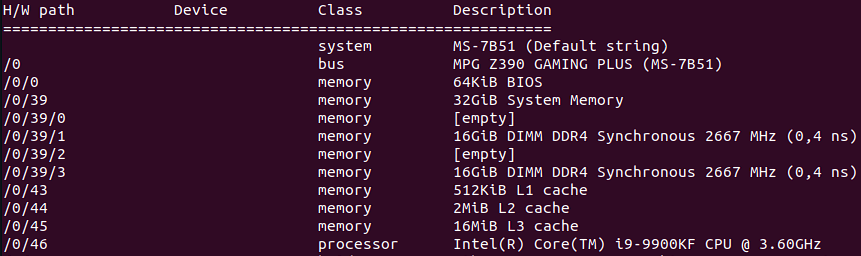
\includegraphics[scale=0.6]{images/Uni_Prozessor.PNG}
	\caption{Systeminformationen Laborrechner}
\end{figure}
Abbildung 2.3 zeigt die Systeminformationen des iCSmini2. Er verfügt über einen Cortex A9 1Ghz Prozessor und über 1GB Arbeitsspeicher.
\begin{figure}[H]
	\centering
	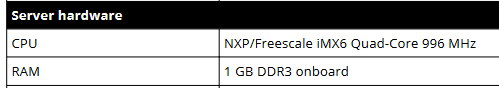
\includegraphics[scale=0.8]{images/Iseg_Prozessor.PNG}
	\caption{Systeminformationen iCSmini2}{Quelle: \url{https://iseg-hv.com/files/media/iseg_manual_iCSmini2_en_20201023133528.pdf} Stand: 09.07.2022}
\end{figure}
\chapter{Evaluation Signaturverfahren}
\section{Vergleich Ed25519 und RSA}
In einer der ersten Vorstellungen von Ed25519 wurde ein Vergleich zu RSA gezogen \cite[Vgl. S.2]{ed25519_paper}. Daraus ging hervor, dass ein 256-Bit Ed25519 public-key ungefähr so sicher wäre, wie ein 3000-Bit RSA public-key. Die beiden Verfahren sind sich also ähnlich in ihrem Sicherheitsaspekt. Ein RSA public-key könnte zwar größer gewählt werden, um das Ermitteln des Schlüssels noch weiter zu erschweren, jedoch gelten die bereits genannten Größen schon als unknackbar. Die dadurch gebotene Sicherheit wäre also nur minimal, während die Berechnungszeit weiterhin ansteigt. Deswegen sollen nun RSA und Ed25519 in ihrer Berechnungszeit verglichen werden. Dabei sollen ein 256-Bit public-key für Ed25519 und ein 3072-Bit public-key für RSA angewendet werden. Zum Bestimmen der Zeit wurde eine 159Mb Iseg Firmwareaktualisierung auf dem iCSmini2 mithilfe des \texttt{time} Befehls 100 Mal verifiziert. Das Verifizieren ist dabei einzige Priorität, da die Schlüsselerzeugung und das Signieren nicht beim Endkunden auf dem iCSmini2 stattfinden und diese somit keiner Zeiteinschränkung unterliegen. Außerdem wurden die Schlüsselerzeugung, das Signieren und das Verifizieren über GPG durchgeführt, welches in einem späteren Kapitel noch genauer vorgestellt werden soll.
\\[1cm]
Wie in Abbildung 3.1 zu sehen ist, benötigte der iCSmini2 12 Minuten und 18,602 Sekunden für 100 Verifizierungen. Dies entspricht einer Rate von 7,38602 Sekunden pro Verifizierung.
\begin{figure}[H]
	\centering
	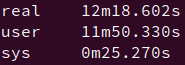
\includegraphics[scale=0.8]{images/ICSMINIII_GPG.PNG}
	\caption{Zeitaufwand Ed25519}
\end{figure}

Für 100 Verifizierungen mit RSA brauchte der iCSmini2, in Abbildung 3.2 zu sehen, 12 Minuten und 26,595 Sekunden. Daraus ergeben sich 7,46595 Sekunden pro Verifizierung.  
\begin{figure}[H]
	\centering
	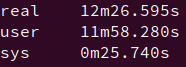
\includegraphics[scale=0.8]{images/ICSMINIRSA.PNG}
	\caption{Zeitaufwand RSA}
\end{figure}
\newpage
\section{Vergleich Ed25519 und Ed448}
Ed448 basiert wie Ed25519 auf EdDSA, verwendet dabei allerdings die Curve448 und die dazugehörigen Parameter für Berechnungen. Die genauen Parameter sind im RFC 8032 \cite[Vgl. S.15-19]{ed25519} zu finden. Durch die veränderte Herangehensweise bietet Ed448 mit einem 224-Bit Sicherheitslevel \cite[Vgl. S.3]{ed25519} eine höhere Sicherheit, da Ed25519, wie bereits erwähnt, auf ein 128-Bit Sicherheitslevel abzielt. Im Austausch für die höhere Sicherheit kostet das Berechnen einer Signatur mit Ed448 auch mehr Resourcen, wie in den Benchmarks von SUPERCOP \cite{ed448} zu sehen ist. So braucht Ed448 1,5 bis 5 Mal mehr Zyklen als Ed25519, um eine Signatur zu verifizieren. Da die Sicherheit mit Ed25519 bereits mehr als ausreichend ist und Resourcen auf den Iseg Geräten knapp sind, wird Ed448 keine Verwendung finden.
\section{Entscheidung}
Wie in 3.1 beschrieben sind sich RSA und Ed25519 in ihrem Sicherheitslevel sehr ähnlich. Durch die Zeittests stellte sich heraus, dass eine Signatur mit Ed25519 schneller verifiziert werden kann als mit RSA.
Dieser Unterschied von $\sim$0,05 Sekunden ist zwar nur marginal, spricht aber dennoch für Ed25519, da jedes noch so kleine Zeitersparnis wichtig ist. Daher soll Ed25519 implementiert werden.  
\chapter{Implementierung}
\section{Python}
Zu Beginn der Arbeit wurde eine mögliche Umsetzung des Signatur- und Verifizierungsverfahrens in Python angestrebt. Eine Lösung hierfür fand sich in {\href{https://pypi.org/project/PyNaCl/}{PyNaCl}. PyNaCl bietet eine Python Anbindung zur \href{https://github.com/jedisct1/libsodium}{libsodium} Bibliothek, wobei es sich um einen portablen fork der \href{https://nacl.cr.yp.to/}{NaCl} (Networking and Cryptograhpy library) handelt. Somit ermöglicht PyNaCl die Verwendung des Ed25519-Signaturverfahrens in Python. Nach ersten Versuchen wurden die Arbeiten an dieser Implementierung jedoch eingestellt, da es sich herausstellte, dass ein Echtwelteinsatz sehr unwahrscheinlich sein wird. PyNaCl fordert eine Python Version von 3.6 oder höher, wobei auf den Geräten von Iseg derzeit maximal Python 3.5 vorzufinden ist. Ein Upgrade der Python Version wäre möglich, hat aber derzeit keine Priorität. 
	\\[1cm]
	Es ist unklar, ob sich ein weiterer Blick in PyNaCl lohnt, falls Python auf den Iseg Geräten nachgerüstet werden sollte. Python unterliegt dem Stigma, langsamere Ausführungszeiten zu haben, da Python-Code erst während der Laufzeit interpretiert wird. Welche Auswirkungen dies genau auf das Verifizieren einer Signatur hat, lässt sich nicht vorher sagen. Somit bleibt eine Umsetzung in Python zukünftig offen. Es müsste aber vorher getestet werden, ob überhaupt ein Zeitersparnis möglich ist und diese Implementierung sinnig wäre.
	\section{C}
	Implementierungen von Ed25519 wurden ursprünglich \cite{edcrypto} in Assembler für amd64 Architektur und in C bereitgestellt. Diese wurden im SUPERCOP \cite{SUPERCOP} toolkit verwendet.
	SUPERCOP wird eingesetzt, um die Leistungsfähigkeit verschiedenster Kryptografiealgorithmen auf unterschiedlicher Hardware zu testen.
	Im Zuge dessen wurde die alte C Implementierung \enquote{ref} verbessert und eine weitere Implementierung namens \enquote{ref10} entwickelt, welche bessere Leistung verspricht. Eine portable Implementierung \cite{github}, welche auf dieser \enquote{ref10} Implementierung basiert, wurde für dieses Projekt verwendet. Die Anwendung soll nun vorgestellt werden.
	\\[1cm]
	Es wird als unsigniertes character-array ein 32-Byte seed, ein 32-Byte public-key, ein 64-Byte private-key und eine 64-Byte Signatur definiert. Die Größe des private-keys ist dabei unterschieldich zur Definition in 2.4, da die Implementierung anders damit verfährt. Zunächst wird der seed zufällig generiert (zum Beispiel unter Linux mit der Hilfe von /dev/urandom). Danach soll die zu signierende Nachricht eingelesen werden, was in diesem Fall die Firmwareaktualisierung darstellt. Die Signierfunktion erwartet dabei einen Input als character-array. Es wird also ein Buffer in Größe der Firmwareaktualisierung vorbereitet, in welchen eben jene Byte für Byte eingelesen wird. 
	\\[1cm]
	Dies kann als problematisch angesehen werden, da hier für eine 200 MB große Aktualisierung auch 200 MB Arbeitsspeicher genutzt werden. Da Iseg Geräte wie der ICS Mini II nur über 1 GB Arbeitsspeicher verfügen, sollte bei größeren Aktualisierungen von dieser Variante abgesehen werden. Eine Optimierung durch Einlesen der Aktualisierung in kleineren Stücken wäre möglich, jedoch erwartet die Signierfunktion die gesamte Nachricht als Argument und müsste dementsprechend auch angepasst werden. Dies stellt sich wiederum als schwierig heraus, da die gesamte Nachricht beim Hashen mit SHA-512 genutzt wird.
	\\[1cm]
	Mithilfe des seeds werden nun public-key sowie private-key generiert. Daraufhin werden der Signaturfunktion die bisher leere Signatur, die Nachricht, die Länge der Nachricht, der public-key und der private-key übergeben. Sie generiert daraus eine Signatur für die Firmwareaktualisierung. Die daraus resultierende Signatur und der public-key werden in eine Datei geschrieben, um beim Verifizieren verwendet werden zu können. Diese Datei muss dabei nicht besonders gesichert sein, da der private-key sich nicht aus der Signatur und dem public-key ermitteln lässt.
	\\[1cm]
	Beim Verifizieren auf der Seite des Nutzers definieren wir erneut als unsigniertes character-array einen 32-Byte public-key und eine 64-Byte Signatur. Aus der oben beschriebenen Datei werden public-key und Signatur gelesen und in die vorbereiteten arrays geschrieben.
	Die zu verifizierende Firmwareaktualisierung wird in einen Buffer eingelesen und danach in ein character-array geschrieben.
	Nun werden der Verifiziermethode die Signatur, die Aktualisierung, die Größe der Aktualisierung und der public-key übergeben und diese entscheidet dementsprechend, ob die Signatur gültig ist oder nicht. Mithilfe des Rückgabewertes der Methode lässt sich so ein Firmwareupdate vorzeitig abbrechen, falls die Signatur ungültig sein sollte.
	
	
	
	\section{GPG}
	\href{https://www.gnupg.org/}{GPG} (GNU Privacy Guard) ist ein kostenloses Kryptographiesystem, welches das Ver- und Entschlüsseln von Daten sowie das Signieren und Verifizieren mit verschieden Signaturalgorithmen ermöglicht. Seit Version 2.1.7 \cite{GNU217} unterstützt GPG auch Signaturen basierend auf Ed25519. Da GPG für kommende Firmwareaktualisierungen für Iseg Geräte eingeplant ist und sich einfach anwenden lässt, lohnt ein Blick auf eine Implementierung mit GPG. 
	\\[1cm]
	GPG bietet dabei mehrere Möglichkeiten für die Darstellung der Signatur. Standardmäßig erzeugt GPG eine \enquote{.gpg}-Datei, welche die signierten Daten sowie die erstelle Signatur enthält. Dies würde in unserem Fall die Firmwareaktualisierung jedoch unbrauchbar machen, falls ein Nutzer eine Installation ohne Überprüfen der Signatur vorzieht, da die \enquote{.gpg}-Datei zwingend verifiziert werden muss, bevor sie weiter genutzt werden kann.
	\\[1cm]
	Wird GPG jedoch beim Signie´ren das Flag \texttt{--detach-signature} mitgegeben, so wird eine separate \enquote{.sig}-Datei erstellt. Somit kann das Update eigenständig angeboten werden. Falls der Nutzer eine Sicherstellung der Integrität der Aktualisierung wünscht, kann er die \enquote{.sig}-Datei herunterladen und dem Updateprozess übergeben.
\section{Einbinden in das Iseg Update-Skript}
Wie bereits in der Vorstellung des Update-Skripts vorgeschlagen, ließen sich die verschiedenen Implementierungen über die Parameterübergabe in das neue Skript einbringen. Dabei wurden zwei neue Parameter definiert, wie in Quelltext 4.1 zu sehen ist. Die Namen der Parameter sollten \texttt{C} für die Implementierung in C und \texttt{G} für die Anwendung von GPG sein. Da der Parameter \texttt{G} schon in Benutzung ist, wurde hier \texttt{S} für \enquote{Signatur} gewählt. Dies ist nur eine Übergangslösung und kann durch passendere Parameternamen ersetzt werden. 
\begin{lstlisting}[language=bash, caption={neue Parameter icsupdate.sh}]
while getopts "nrRhf:p:g:Gs:S:C:" Option ; do
	case $Option in
		S)	GPG_SIG_FILE=$OPTARG
			;;
		C)	C_SIG_FILE=$OPTARG
			;;
	esac
done
\end{lstlisting}
Hierbei wird im Quelltext 4.1 nur ein Ausschnitt aus der Parameterübergabe gezeigt, da die restlichen Parameter für die Erklärung keine Bedeutung hatten.
\texttt{GPG\_SIG\_FILE} und \texttt{C\_SIG\_FILE} bekommen nun also den Namen der Signaturdatei als Wert übergeben. So kann später aus diesen beiden Variablen und der Updatepfadvariable ein vollständiger Pfad erzeugt werden, welcher den einzelnen Implementierungen übergeben werden kann.
\\[1cm]
\subsection*{GPG}
Sollte bei GPG keine separate Signatur erstellt worden sein, so kann die \enquote{.gpg}-Datei einfach mit dem normalen \texttt{f}-Parameter übergeben werden.
\begin{lstlisting}[language=bash, caption={.gpg file handling icsupdate.sh}]
# is ZIP_FILE a signed GPG file (non detached signature)
if [ "${ZIP_FILE: -4}" == ".gpg" ] ; then
\end{lstlisting}
Wie in Quelltext 4.2 zu sehen ist, wird standardmäßig zuerst geprüft, ob die übergebene Firmwareaktualisierung eine GPG-Dateiendung hat. Sollte dies der Fall sein, so wird die Aktualisierung nun verifiziert und entschlüsselt, da \enquote{.gpg}-Dateien vor dem entschlüsseln nicht verwendet werden können.
\newpage
\begin{lstlisting}[language=bash, caption={.gpg Umbenennung icsupdate.sh}]
else
    ZIP_FILE=${ZIP_FILE%.gpg}
    echo "correct signature, resuming update..."
fi
\end{lstlisting}
Ist das Entschlüsseln abgeschlossen so wird \texttt{ZIP\_FILE} so abgeändert, dass die Variable nun den Namen der Firmwareaktualisierung  als Wert zugewiesen bekommt. Somit können alle weiteren Operationen wie üblich verfahren.
\\[1cm]
\begin{lstlisting}[language=bash, caption={GPG Verifizierung icsupdate.sh}]
echo "checking signature..."
	${GPG} --verify "${ZIP_FILE_PATH}${GPG_SIG_FILE}" "${ZIP_FILE_PATH}${ZIP_FILE}" 2>/dev/null
	IS_VALID_SIGNATURE=$?
\end{lstlisting}
Wurde mit dem Parameter \texttt{S} eine GPG Signatur übergeben, so wird, wie in Quelltext 4.4 zu sehen ist, GPG mit dem Parameter \texttt{--verify} aufgerufen und die Signatur \texttt{GPG\_SIG\_FILE} und die Firmwareaktualisierung \texttt{ZIP\_FILE} übergeben. In der Variable \texttt{IS\_VALID\_SIGNATURE} wird der Rückgabewert des Verifiziervorganges hinterlegt. War das Verifizieren erfolgreich so wird die Installation fortgesetzt, anderenfalls wird hier mit einem \texttt{exit 1} das Skript beendet und eine entsprechende Fehlermeldung ausgegeben.
\newpage
\subsection*{C}
\begin{lstlisting}[language=bash, caption={C Verifizierung icsupdate.sh}]
if [ -f "${ZIP_FILE_PATH}${C_SIG_FILE}" ] ; then

	echo "C checking signature..."
	${ZIP_FILE_PATH}${C_VERIFY_FILE} ${ZIP_FILE_PATH}${ZIP_FILE} ${ZIP_FILE_PATH}${C_SIG_FILE}
	IS_VALID_SIGNATURE=$?

	if [ $IS_VALID_SIGNATURE -eq 1 ] ; then
		echo "invalid signature, check the signature 
		file name for errors: 
		${ZIP_FILE_PATH}${C_SIG_FILE}"
		exit 1
	else
		echo "correct signature, resuming update..."
	fi
fi
\end{lstlisting}
Der Codeabschnitt in Quelltext 4.5 zeigt, dass das Einbinden des Verifiziervorganges mit C sehr ähnlich zur GPG Variante ist. Es wird zunächst geprüft, ob eine Signatur mit dem \texttt{C}-Parameter übergeben wurde. In diesem Fall wird probiert die Firmwareaktualisierung zu Verifizieren. Die Variable \texttt{C\_VERIFY\_FILE} enthält dabei den Namen des Verifizierprogrammes. Erneut wird der Rückgabewert des Verifiziervorganges in \texttt{IS\_VALID\_SIGNATURE} hinterlegt. Sollte das Verifizieren fehlschlagen so wird eine entsprechende Fehlermeldung ausgegeben und das Skript beendet. Bei einer gültigen Signatur wird der Erfolg signalisiert und die Installation darf fortfahren.
\chapter{Ergebnis und Zukunft}
\section{Ausführungszeiten}

\noindent
Mithilfe des Linux Befehls \texttt{time} wurden die Verifizierverfahren 100 mal ausgeführt, um daraus einen Mittelwert zu bilden.
\\[1cm]
\subsection*{Laborrechner}
Zunächst sollen die Ergebnisse des Laborrechners dargestellt werden. Für das Verifizieren mit der Implementierung in C benötigte der Rechner 46,329 Sekunden, das entspricht 0,46329 Sekunden pro Verifizierung.
\begin{figure}[H]
	\centering
	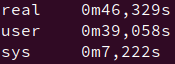
\includegraphics[scale=0.8]{images/Laborrechner_C.PNG}
	\caption{Zeit Laborrechner C}
\end{figure}
\noindent
Das Verifizieren mit GPG auf dem Laborrechner dauerte 55,259 Sekunden, was wiederum 0,55259 Sekunden pro Verifizierung entspricht.
\begin{figure}[H]
	\centering
	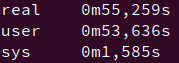
\includegraphics[scale=0.8]{images/Laborrechner_GPG.PNG}
	\caption{Zeit Laborrechner GPG}
\end{figure}
\newpage
\subsection*{iCSmini2}
\noindent
Nun werden die Zeiten des iCSmini2 aufgezeigt. Für das Verifizieren mit der C Implementierung brauchte der iCSmini2 24 Minuten und 51,720 Sekunden, das entspricht 14,9172 Sekunden pro Verifizierung.
\begin{figure}[H]
	\centering
	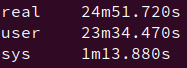
\includegraphics[scale=0.8]{images/ICS_MINI_C_100.PNG}
	\caption{Zeit iCSmini2 C}
\end{figure}
Das Verifizieren mit GPG dauerte 12 Minuten und 18,602 Sekunden mit dem iCSmini2. Diese Zeit ergibt eine durchschnittliche Ausführungszeit von 7,38602 Sekunden pro Verifizierung.
\begin{figure}[H]
	\centering
	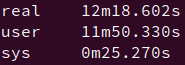
\includegraphics[scale=0.8]{images/ICSMINIII_GPG.PNG}
	\caption{Zeit iCSmini2 GPG}
\end{figure}
\newpage
\section{Vergleich und Auswahl eines Verfahrens}
Das Verifizieren mit GPG schließt mit 7 Sekunden in einem passablen Zeitumfang ab. Dennoch würden 7 Sekunden eine merkbare Wartezeit im Aktualisierungsprozess darstellen. Eine mögliche Optimierung findet sich in der C-basierten Implementierung. Diese nimmt zwar im Durchschnitt 14-15 Sekunden in Anspruch, könnte wahrscheinlich aber verbessert werden. 13 Sekunden werden allein für das Hashen der Aktualisierungsdatei verwendet. Ein Austauschen des Hashingalgorithmus SHA-512 durch eine Implementierung von SHA-512 in ARMv7 Assembler könnte hier Abhilfe schaffen. Es ist unklar, ob der Verifiziervorgang damit auf unter 7 Sekunden gebracht werden könnte, aber es ist der beste Lösungsansatz.
\\[1cm]
Zum derzeitigen Stand wäre die Umsetzung mit GPG die schnellste Lösung und wird somit mit großer Wahrscheinlichkeit auch Anwendung finden.
\section{Verwendung durch den Nutzer}
Es sollte diskutiert werden, wie Aktualisierung, Signatur und public-key künftig beim Nutzer ankommen. Die Aktualisierung wurde bisher standardmäßig online \cite{IsegDL} zum Download angeboten. Hierfür gibt es mehrere Ideen. Beim GPG Verfahren muss zudem der public-key als vertrauenswürdiger Schlüssel eingerichtet sein. Dies könnte auch automatisch beim Aktualisieren geschehen und erfordert nicht zwingend eine Aktion des Nutzers. Folgende Vorschläge, welche einen public-key spezifisch ansprechen, thematisieren eine Implementierung in C.
\\[1cm]
Zunächst könnten Signatur und public-key im selben Downloadverzeichnis, wie die Aktualisierung, angeboten werden. So würde es auf den Nutzer zurückfallen, sich aktiv die Signatur zu beschaffen. Würde er dies nicht machen, so würde die Aktualisierung auch ohne Signatur funktionieren, jedoch dann auf Risiko des Nutzers. Für ein Verfahren mit Verifizierung muss dem Nutzer eine einfache Möglichkeit im Webinterface geboten werden, um die Signatur und den Public Key im Update-Verzeichnis (/mnt/user/data/updates) zu hinterlegen und das Update-Skript mit entsprechenden Parametern aufzurufen.
\\[1cm]
Des Weiteren besteht die Möglichkeit, sämtliche benötigten Dateien in einem Tarball anzubieten. Dieser könnte heruntergeladen und vom Update-Skript vor der Installation entpackt werden. Somit müsste sich der Kunde nur um eine Datei aktiv kümmern, der Rest geschieht automatisch. Diese Möglichkeit würde allerdings die verifizierte Aktualisierung auf den Nutzer forcieren, da die Signatur automatisch verarbeitet wird. Hier müsste gegebenenfalls eine Eingabe des Nutzers angefordert werden, ob er die Aktualisierung gegen die Signatur prüfen will.
\\[1cm]
Durchaus vorstellbar wäre auch die Signatur und Aktualisierung im GPG Signaturverfahren zu einer \enquote{.gpg}-Datei zu kombinieren. Vorteil dieser Methode ist, dass der Kunde nur, wie gewohnt, eine Datei herunterladen muss. Allerdings wird so ein Verifizieren erzwungen, da die \enquote{.gpg}-Datei vorher nicht als Aktualisierung genutzt werden kann. Dies könnte zu Problemen führen, falls ein Kunde keine Verifizierung möchte. Außerdem besteht die Möglichkeit, dass ein Kunde seine iCS Version so weit herunterstuft, dass er kein GPG mehr auf dem Gerät zur Verfügung hat. In solch einem Fall muss ein Update auch in ursprünglicher Form zum Download bereitstehen und nicht nur als \enquote{.gpg}-Datei.
\\[1cm]
Es könnte sich anbieten, bei erfolgreicher Verifizierung eine Art Flag in einer Log-Datei zu hinterlegen. Somit könnte gegen Nutzer vorgegangen werden, welche die Schuld für ihr nicht funktionierendes System in einer fehlerhaften Aktualisierung suchen. Wäre dieses Flag gesetzt, müsste die Installation mit einer unversehrten Datei abgelaufen sein und das System einwandfrei laufen (vorrausgesetzt, die Aktualisierung war nicht von vorneherein fehlerhaft).
So können die Probleme nur vom Nutzer verursacht worden sein.
\\[1cm]
Das in der Aufgabenstellung besprochene visuelle Feedback für den Nutzer wurde nicht bearbeitet. Der zur Verfügung gestellte iCSmini2 besitzt kein Display, somit wäre ein Testen dieser Funktion zunächst nicht möglich gewesen. Sollten technische Daten über Iseg Geräte mit Displays vorliegen, so könnte das Update-Skript angepasst werden. Die entsprechenden Fallunterscheidungen von Erfolg und Misserfolg beim Verifizieren müssten nur durch eine visuelle Ausgabe des Ergebnisses ergänzt werden.
\section{Fazit}
Mehrere Softwarelösungen für das Signieren und Verifizieren von Firmwareaktualisierungen der Firma Iseg konnten entwickelt werden.
Hierbei wurde durch das Testen verschiedener Implementierungen eine Umsetzung von Ed25519 über GPG, aufgrund ihrer Geschwindigkeit, als beste Variante determiniert.
Die Implementierung von Ed25519 in C zeigt Potenzial und könnte GPG ersetzen, sofern ein besser Hashing-Algorithmus gefunden werden kann.

Da das Verifizieren Teil des \enquote{icsupdate.sh} Update-Skripts geworden ist, hat sich für den Kunden nichts merklich am Aktualisierungsprozess geändert. Außerdem besteht weiterhin die Möglichkeit, Firmware auch ohne Signatur zu installieren.

Es stellt kein Problem dar, dass sich die Iseg Geräte bereits im ausgelieferten Zustand befinden, da die Softwarelösung in C per Yocto-Layer nachgeliefert werden könnte. GPG ist bereits installiert, lediglich der passende public-key muss als trusted-key auf dem System hinterlegt sein.

Somit konnte für alle gestellten Aufgaben, außer dem visuellen Feedback einer Verifizierung, eine mögliche Lösung gefunden werden. Kam es zu Problemen, so konnte meist eine mögliche Lösung für die Zukunft vorgeschlagen werden, wie zum Beispiel der neue Hashing-Algorithmus für die C Implementierung.
\section{Ausblick}
Eine Signatur im Ed25519-Signaturverfahren bietet derzeit ausreichend Schutz für das Sicherstellen der Integrität einer Iseg Firmwareaktualisierung. Dieser Schutz ist gegeben durch das Problem des diskreten Logarithmus. Der public-key lässt sich relativ leicht durch diskrete Epxonentiation aus einem private-key zu errechnen. Für die Umkehrfunktion der diskreten Exponentialfunktion, den diskreten Logarithmus, ist jedoch kein effizienter Algorithmus zur Berechnung bekannt. Dies macht es einem Angreifer sehr schwer, den private-key zu berechnen. Er müsste mit den besten bekannten Algorithmen einen Aufwand von \begin{math}O(2^{128})\end{math} \cite[Vgl. S.1]{ed25519_paper} erbringen, um womöglich den private-key zu ermitteln. Für unseren Anwendungsfall ist es unwahrscheinlich, dass ein Angreifer weder genügend Rechenleistung aufbringen kann noch möchte, um dies in einem sinnvollen Zeitraum durchzuführen. Durch Wechseln des private-keys für jede neue Firmware-Version könnte dies noch weiter erschwert werden.
\\[1cm]
Sollte ein Quantencomputer mit ausreichend Anzahl an Qubits entwickelt werden, so wäre das Signieren mit Ed25519 nichtig, da mithilfe des Shor-Algorithmus \cite{SHOR} für Quantencomputer das zuvor genannte Problem trivialisiert werden kann. In diesem Fall bietet sich ein Umstieg auf symmetrische Signaturverfahren an, deren Sicherheit nicht durch die Existenz eines Quantencomputers beeinträchtigt ist. Als Beispiel lässt sich dafür AES-256 aufführen.

\appendix % Anhang
\chapter{CD}
Der Arbeit liegt eine CD bei, welche sämtlichen Programmcode enthält. Dabei handelt es sich um die C Implementierung im Ordner \enquote{C} sowie den Bash Code, welcher als Teil des editierten icsupdate.sh existiert. Außerdem findet sich darauf eine Anleitung zum Verwenden der verschiedenen Implementierungen.
\chapter{C Programmcode}
\section{Schlüsselerstellung und Signieren}
\begin{lstlisting}[language=C]
#include "ed25519.h"
#include <stdio.h>
#include <stdlib.h>
#include <string.h>
int main(int argc, char *argv[]) {

unsigned char seed[32], public_key[32], private_key[64], signature[64];
long FILE_SIZE;
char *BUFFER;


// open update file and read it into a BUFFER

FILE *UPDATE_FILE = fopen ( argv[1], "rb" );
if ( !UPDATE_FILE ) perror(argv[1]), exit(1);

fseek( UPDATE_FILE , 0L , SEEK_END);
FILE_SIZE = ftell( UPDATE_FILE );
rewind( UPDATE_FILE );
BUFFER = calloc( 1, FILE_SIZE + 1 );
if ( !BUFFER ) fclose(UPDATE_FILE), fputs("memory alloc 
   fails", stderr), exit(1);

if ( 1 != fread( BUFFER , FILE_SIZE, 1 , UPDATE_FILE) )
fclose(UPDATE_FILE), free(BUFFER), fputs("entire read fails", stderr), exit(1);
fclose(UPDATE_FILE);

// write update file from BUFFER to char array

unsigned char *message = malloc(FILE_SIZE + 1 );

if (message == NULL) {
printf("error while allocating memory for update file");
free(BUFFER);
exit(1);
}

for (int i = 0; i < FILE_SIZE; ++i) {
message[i] = ((char *)BUFFER)[i];
}

free(BUFFER);

if (ed25519_create_seed(seed)) {
printf("error while generating seed\n");
exit(1);
}

ed25519_create_keypair(public_key, private_key, seed);

ed25519_sign(signature, message, FILE_SIZE, public_key, private_key);

free(message);


/*  splitting key creation and signing process:
- after ed25519_create_keypair, write public_key and 
  private_key to any file
- in a separate program (signing) : load public_key 
  private_key and the update file ("message") into char arrays
- file size of the update file and an empty 
  64 Byte char array (signature) are needed
- call ed25519_sign and pass the prepared parameters
- write public_key and signature to any file
- file size should be 96 Byte (32 Byte public_key + 64 Byte 
  signature in that specific order)
*/

// write signature and public key to given file

FILE *KEY_SIG_FILE = fopen(argv[2], "wb+");
if (KEY_SIG_FILE == NULL)
{
printf("error opening file\n");
exit(1);
}
for (int i= 0; i < sizeof(public_key); i++) {
fputc(public_key[i], KEY_SIG_FILE);
}
for (int i= 0; i < sizeof(signature); i++){
fputc(signature[i], KEY_SIG_FILE);
}

fclose(KEY_SIG_FILE);

return 0;
}	
\end{lstlisting}
\section{Verifizieren}
\begin{lstlisting}[language=C]
#include "ed25519.h"
#include <stdio.h>
#include <stdlib.h>
#include <string.h>
#include <time.h>
int main(int argc, char** argv) {

// public key has to be 32-Byte writable char array
// signature has to be 64-Byte writable char array

long FILE_SIZE;
char *BUFFER;
unsigned char PUBLIC_KEY[32], SIGNATURE[64];


// load public key and signature

FILE *SIGNATURE_FILE = fopen ( argv[2] , "rb" );
if ( !SIGNATURE_FILE ) {
perror(argv[2]), exit(1);
}

fseek( SIGNATURE_FILE , 0L , SEEK_END);
FILE_SIZE = ftell( SIGNATURE_FILE );

// "SIGNATURE_FILE" has to be 96 Bytes 
   ((public_key)32+64(signature))
if (FILE_SIZE != sizeof(PUBLIC_KEY)+sizeof(SIGNATURE)) 
   fclose(SIGNATURE_FILE), fputs("incompatible signature 
   type\n", stderr), exit(1); 

rewind( SIGNATURE_FILE );

BUFFER = calloc( 1, FILE_SIZE + 1 );
if ( !BUFFER ) fclose(SIGNATURE_FILE), fputs("memory alloc 
   fails", stderr), exit(1);

if ( 1 != fread( BUFFER , FILE_SIZE, 1 , SIGNATURE_FILE) )
fclose(SIGNATURE_FILE), free(BUFFER), fputs("entire read 
fails", stderr), exit(1); fclose(SIGNATURE_FILE);

// write public key and signature to respective variables

for (int i = 0; i < FILE_SIZE; ++i) {
if ( i < sizeof(PUBLIC_KEY)) {
PUBLIC_KEY[i] = ((char *)BUFFER)[i];
}
else 
SIGNATURE[i-sizeof(PUBLIC_KEY)] = ((char *)BUFFER)[i];
}

free(BUFFER);

// load update file

FILE *UPDATE_FILE = fopen ( argv[1], "rb" );
if ( !UPDATE_FILE ) perror(argv[1]), exit(1);

fseek( UPDATE_FILE , 0L , SEEK_END);
FILE_SIZE = ftell( UPDATE_FILE );
rewind( UPDATE_FILE );

BUFFER = calloc( 1, FILE_SIZE + 1 );
if ( !BUFFER ) fclose(UPDATE_FILE), fputs("memory alloc for 
reading in the update file failed", stderr), exit(1);

if ( 1 != fread( BUFFER , FILE_SIZE, 1 , UPDATE_FILE) )
fclose(UPDATE_FILE), free(BUFFER), fputs("reading of update 
file failed", stderr), exit(1); fclose(UPDATE_FILE);

unsigned char *message = malloc(FILE_SIZE + 1 );

if (message == NULL) {
printf("error while allocating memory for update file");
free(BUFFER);
exit(1);
}

for (int i = 0; i < FILE_SIZE; ++i) {
message[i] = ((char *)BUFFER)[i];
}
free(BUFFER);

// verify integrity of update file

if (ed25519_verify(SIGNATURE, message, FILE_SIZE, PUBLIC_KEY)) {
printf("\nvalid signature\n");
return 0;
} else {
printf("\ninvalid signature\n");
return 1;
}
free(message);


}
\end{lstlisting}
\chapter{Bash Programmcode}
\section{Variablendeklaration}
\begin{lstlisting}[language=bash]
GPG=`command -v gpg` || { echo >&2 "Update ERROR: Program gpg 
not available.  Aborting."; exit 1; }
	
	# START
	
	ZIP_FILE_PATH="/mnt/user/data/updates/"
	ZIP_FILE=""
	GPG_SIG_FILE=""
	C_SIG_FILE=""
	C_VERIFY_FILE="verify_file_arm"
	IS_VALID_SIGNATURE=""
	while getopts "nrRhf:p:g:Gs:S:C:" Option ; do
		case $Option in
			n)	NO_RECURSE=1
				;;
			r) 	FactoryReset
				exit 0
				;;
			R) 	FactoryReset full
				exit 0
				;;
			h) 	Usage
				# Exit if only usage (-h) was 
				  specfied.
				if [ "$#" -eq 1 ] ; then
					exit 10
				fi
				exit 0
				;;
			f)	ZIP_FILE=$OPTARG
				;;
			p)	ZIP_FILE_PATH=$OPTARG
				;;
			g)	ISEG_SERIAL=$OPTARG
				GetDeviceType ${ISEG_SERIAL}
				exit 0
				;;
			G)	GetDefaultDeviceType
				exit 0
				;;
			s)	SET_CONFIGURATION=$OPTARG
				SetConfiguration "/" ${SET_CONFIGURATION}
				exit 0
				;;
			S)	GPG_SIG_FILE=$OPTARG
				;;
			C)	C_SIG_FILE=$OPTARG
				;;
		esac
	done
	
	if [ "$ZIP_FILE" = "" ] ; then
		Usage
		exit 0
	fi
	
	# is ZIP_FILE an existing file?
	if [ ! -r "${ZIP_FILE_PATH}${ZIP_FILE}" ] ; then
		echo >&2 "Update ERROR: 
		${ZIP_FILE_PATH}${ZIP_FILE} does not exist 
		or cannot be read, exiting"
		exit 1
	fi	
\end{lstlisting}
\section{Verifizieren mit GPG}
\begin{lstlisting}[language=bash]
# is ZIP_FILE a signed GPG file? (non detached signature)
	if [ "${ZIP_FILE: -4}" == ".gpg" ] ; then
	
		echo "checking signature..."
		${GPG} --yes --output "${ZIP_FILE_PATH}
		${ZIP_FILE%.gpg}" --decrypt "${ZIP_FILE_PATH}
		${ZIP_FILE}" 2>/dev/null
		IS_VALID_SIGNATURE=$?
	
		if [ $IS_VALID_SIGNATURE -eq 1 ] ; then
			echo "incorrect GPG signature, check 
			the signature file name for errors: 
			${ZIP_FILE_PATH}${ZIP_FILE}"
			exit 1
		elif [ $IS_VALID_SIGNATURE -eq 2 ] ; then
	    		echo "invalid GPG signature,
	    		check the signature file 
	    		name for errors: 
	    		${ZIP_FILE_PATH}${ZIP_FILE}"
	        	exit 1
	    else
	    	  ZIP_FILE=${ZIP_FILE%.gpg}
	    	  echo "correct signature, resuming update..."
	    fi
	fi
	
	# if a GPG_SIG_FILE was provided, check if it is a
	  valid GPG signature
	if [ -f "${ZIP_FILE_PATH}${GPG_SIG_FILE}" ] ; then
	
		if [ "${GPG_SIG_FILE: -4}" == ".gpg" ] ; then
			echo "pass .gpg files only 
			as argument to the -f parameter"
			exit 1
		fi
	
		echo "checking signature..."
		${GPG} --verify "${ZIP_FILE_PATH}
		${GPG_SIG_FILE}"
		"${ZIP_FILE_PATH} ${ZIP_FILE}" 2>/dev/null
	    	IS_VALID_SIGNATURE=$?
	
		if [ $IS_VALID_SIGNATURE -eq 1 ] ; then
			echo "incorrect GPG signature, 
			check the signature file name for 
			errors: 
			${ZIP_FILE_PATH}${GPG_SIG_FILE}"
			exit 1
	
		elif [ $IS_VALID_SIGNATURE -eq 2 ] ; then
	    		echo "invalid GPG signature, check the 
	    		signature file name for errors: 
	    		${ZIP_FILE_PATH}${GPG_SIG_FILE}"
	        	exit 1
	    	else
			echo "correct signature, 
			resuming update..."
		fi
	fi	
\end{lstlisting}
\newpage
\section{Verifizieren mit C Implementierung}
\begin{lstlisting}[language=bash]
# if a C_SIG_FILE (signature generated by ed25519 c program) 
was provided, check if it is a valid signature
	if [ -f "${ZIP_FILE_PATH}${C_SIG_FILE}" ] ; then
	
		echo "C checking signature..."
		${ZIP_FILE_PATH}${C_VERIFY_FILE} ${ZIP_FILE_PATH}${ZIP_FILE} ${ZIP_FILE_PATH}${C_SIG_FILE}
		IS_VALID_SIGNATURE=$?
	
		if [ $IS_VALID_SIGNATURE -eq 1 ] ; then
			echo "invalid signature, check the 
			signature file name for errors: 
			${ZIP_FILE_PATH}${C_SIG_FILE}"
			exit 1
		else
			echo "correct signature, 
			resuming update..."
		fi
	fi
	exit 0
\end{lstlisting}
\bibliographystyle{plain}
\bibliography{refs.bib}
\end{document}